
\subsection{Meldeprint}
%HIER SCHREIBT CLAUDIUS
Die Software des Meldeprints ist in drei Bereiche unterteilt. Beinahe die ganze Überwachung der Module kann in einem Bereich abgehandelt werden. Die anderen beiden dienen zum einen für die Anzeige und die Initialisierung und zum anderen für die Aktualisierung der eingehenden Daten.

\begin{figure}[htbp] 
  \centering
     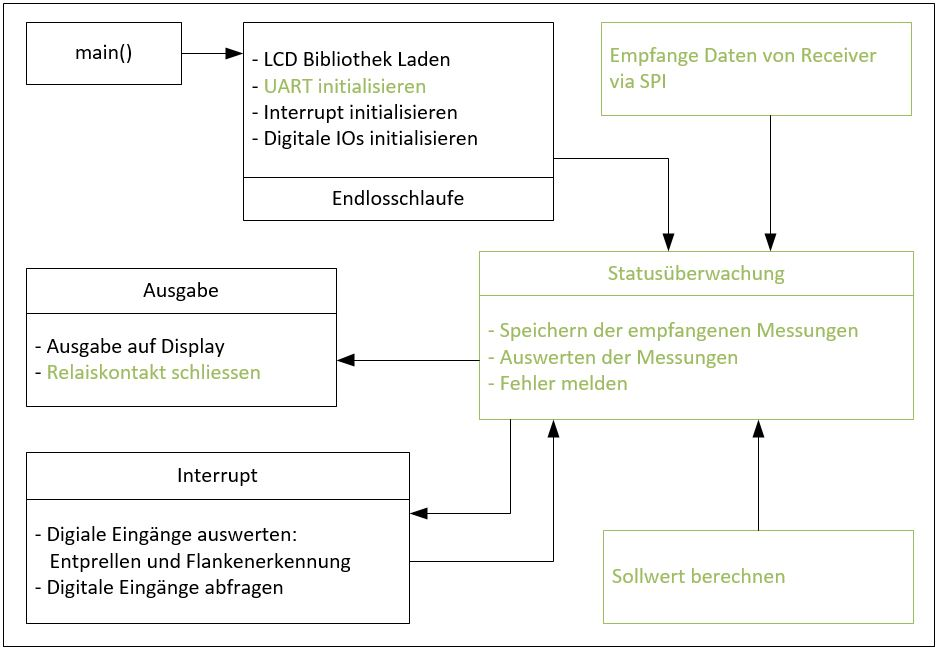
\includegraphics[width=1\textwidth]{graphics/reportboard-software-river}
  \caption{Visualisierung Softwarekonzept}
  \label{fig:reportboard-software-river}
\end{figure}

Wie die Bereiche der Software zusammenarbeiten ist in Abbildung \ref{fig:reportboard-software-river} gut ersichtlich. In der Initialisierung werden als erstes die Hardwarekomponenten und Interrupts initialisiert, dann wird die Endlosschlaufe aufgerufen.
\newline
Der initialisierte Timer Interrupt ruft dann alle 15$u$s die Routine auf, die den Receiver nach Daten abfragt und die digitalen Eingänge entprellt und eine Flankendetektion durchführt.
\newline
Die Endlosschlaufe ruft eine Routine auf, die jeweils eingegangene Daten, der gemessenen Spannung, mit der Identifikationsnummer der Sensorprints in ein Array speichert und mit dem Sollwert vergleicht. Der Sollwert entspricht dem arithmetischen Mittelwert der Spannungen dieses einen Strings von Modulen. Bei einer Abweichung von 20 Prozent, wird dasjenige Modul vorgemerkt. Falls nach einer weiteren Messung die Spannung des selben Moduls gleich vom Mittelwert abweicht, muss ein Fehler gemeldet werden. Die Identifikationsnummer wird auf dem Display angezeigt. Der ganze Prozess vom Start des Meldeprints bis zur Fehlermeldung werden hier weiter vertieft behandelt.
\todo{ich würde nach der einleitung des meldeprints keine subsection machen für das flussdiagramm}

\subsubsection{Inbetriebnahme}
%HIER SCHREIBT CLAUDIUS
Bei der Inbetriebnahme werden als erstes die Peripheriegeräte initialisiert. Darunter befinden sich der LCD Display und der Receiver. Weiter muss die UART Kommunikation und der Timer Interrupt initialisiert werden. In der Endlosschlaufe des Hauptprogramms werden dann die ganzen Daten der Sensorplatine gespeichert und in einem Array Register gespeichert und weiterverarbeitet.

\subsubsection{Receiver}
%HIER SCHREIBT CLAUDIUS
Der Receiver detektiert über einen Ferrit-Kern über der DC-Leitung des Strings die Signale der Sensorplatine. Die Datenpakete werden mit der Identifikationsnummer und der Prüfsumme an den Mikrocontroller weitergeleitet. Diese Kommunikation soll auf SPI basieren. Die Checksum soll ausgewertet werden. Detektiert diese keine Übertragungsfehler, sollen die Informationen weiter verarbeitet werden. Ansonsten wird eine weitere Sendung derjenigen Sensorplatine abgewartet. \\

\subsubsection{Fehlererkennung}
Wird ein defektes oder beschmutztes Spannungsmodul detektiert wird eine entsprechende Fehlermeldung auf dem Display ausgegeben. Zusätzlich zu dieser Information sollen die Identifikationsnummer und der allfällige Name des Panels ausgegeben werden. \\
Ist der allgemeine Mittelwert über zwei Stunden tief, wird darauf geschlossen, dass Dunkelheit herrscht. In dieser Situation wird keine Fehlermeldung ausgegeben.



wieso-was-wie-unter welchen Bedingungen
\subsubsection{Fehlermeldung}
Die Fehlermeldung besteht aus der Fehlerankündigung selbst und der Identifikationsnummer der Sensorplatine, welche am defekten oder verschmutzten Modul befestigt ist. Die Fehlerankündigung ist als Text wie beispielsweise "Problem beim Modul..." auf dem Display zu sehen. Die Identifikationsnummer des Moduls wird von einer 8bit Binärzahl in eine Dezimalzahl umgewandelt und so angezeigt.

wieso-was-wie-unter welchen Bedingungen
\subsubsection{Benutzerinterface}
Das Menu und der Drehgeber bilden zusammen eine einfache Schnittstelle zwischen Mensch und Maschine. In der Abbildung \todo{Abbildung Menü} ist der Aufbau des Menus abgebildet. 
Das Menu ist, wie in der Abbildung \todo{Abbildung Menü}  ersichtlich, in drei Ebenen eingeteilt.










